\begin{figure}[H]
	\centering
\begin{tikzpicture}[node distance=2.5cm,auto,>=latex']



\tikzstyle{int}=[draw, fill=blue!20, minimum size=2em]
\tikzstyle{init} = [pin edge={to-,thin,black}]

\tikzstyle{sensor}=[draw, fill=blue!20, text width=7em, 
text centered, minimum height=5em,drop shadow]
\tikzstyle{ann} = [above, text width=5em, text centered]
\tikzstyle{wa} = [sensor, text width=8em, fill=red!20, 
minimum height=6em, rounded corners, drop shadow]
\tikzstyle{sc} = [sensor, text width=13em, fill=red!20, 
minimum height=10em, rounded corners, drop shadow]

\node (wa) [wa]  {Fluid Dynamics};
\path (wa.east)+(+2.5,0) node (force) [sensor] {Surface Force Calculation};
\path [draw, ->] (wa.east)  -- node [] {}  (force.west);
\path (force.south)+(0,-2.5) node (structure) [wa] {Multi-body Dynamics};
\path [draw, ->] (force.south)  -- node [] {}  (structure.north);
\path (structure.west)+(-2.5,0) node (disp) [sensor] {Displacement Calculation};
\path [draw, ->] (structure.west)  -- node [] {}  (disp.east);
\path [draw, ->] (disp.north)  -- node [] {$t_{l+1}=t_{l}+\Delta t$}  (wa.south);
\node[inner sep=0pt] at (-6,-1.7)
{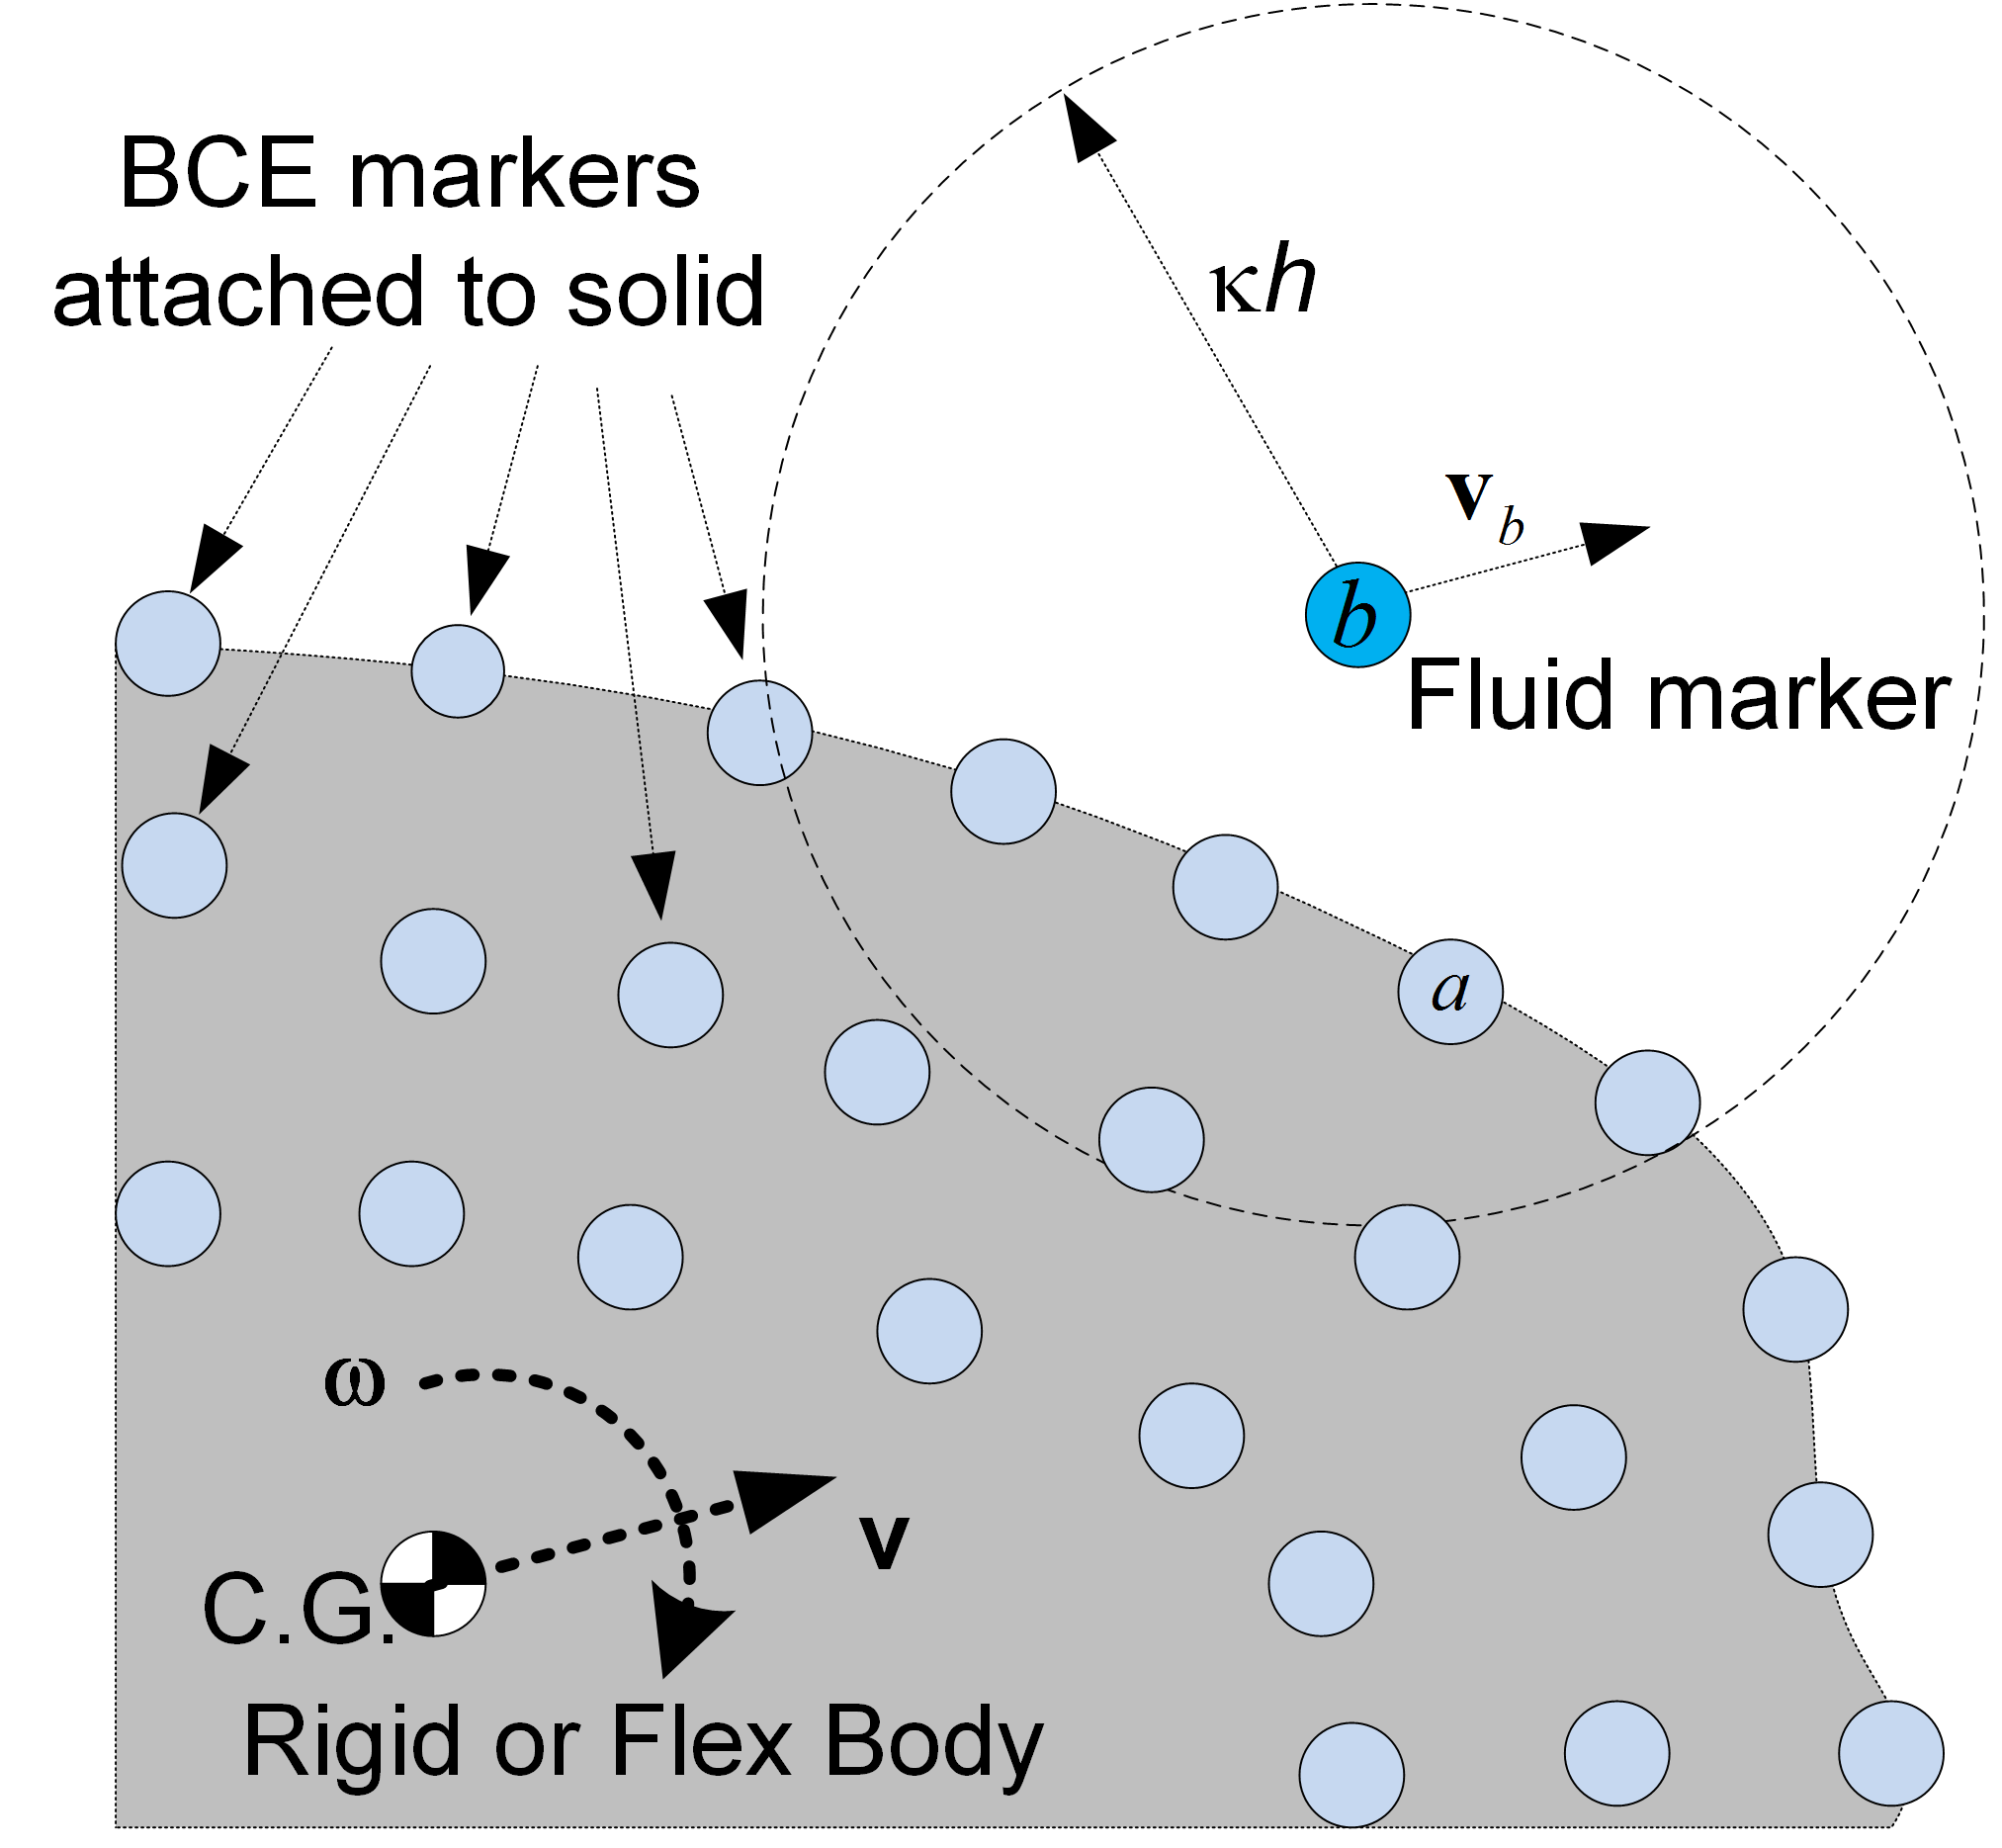
\includegraphics[width=0.42\textwidth]{images/BCE.png}};



\end{tikzpicture}
\caption{Explicit coupling between the structure and the fluid systems through BCE markers. Multiple rows of BCE markers are placed on  solid objects and they are used to enforce no-slip boundary condition. BCE trasnfer the surface forces from the fluid sub-system to the solid sub-system. The position, velocity and acceleration of these markers are dictated by their associated solid object.}
\end{figure}